\subsection*{\lr{2.6.4} بهبود کارایی الگوریتم}
  الگوریتم ساخت جدول معنایی «قطعی» نیست: در اکثر مراحل، انتخاب برگ برای گسترش و در صورتی که برگ بیش از یک فرمول غیرلفظی داشته باشد، انتخاب فرمول برای تجزیه آزاد است. این امکان را فراهم می‌کند که از \emph{هدایت‌کننده‌ها} (heuristics) استفاده کنیم تا جدول سریع‌تر تکمیل شود. همان‌طور که در بخش \lr{2.6.2} دیدیم، بهتر است ابتدا \emph{$\alpha$-فرمول‌ها} را باز کنیم و سپس \emph{$\beta$-فرمول‌ها} تا از تکرار بیهوده جلوگیری گردد.
  
  \paragraph{کوتاه‌سازی جدول با بستن زودهنگام شاخه: }
  می‌توان یک شاخه را به‌محض آنکه شامل یک فرمول و متمم آن شود (نه صرفاً یک زوج متمم از لفظ‌ها) بست. واضح است که ادامهٔ گسترش گره‌ای که برچسب
  \[
  \{\,p \land (q \lor r),\;\neg\bigl(p \land (q \lor r)\bigr)\}
  \]
  را دارد بی‌معنی است. اثبات اینکه این تغییر در صحت الگوریتم خللی ایجاد نمی‌کند به‌عنوان تمرین باقی گذاشته شده است.
  
  \paragraph{کاهش تکرارِ بازنویسی فرمول‌ها: }
  انتقال مکرر فرمول‌ها از یک گره به گرهٔ فرزند:
  \[
  U(l') = \bigl(U(l)\setminus\{A\}\bigr)\;\cup\;\{A_1,A_2\}
  \]
  منجر به تکرارهای بیهوده می‌شود. در گونه‌ای از جدول معنایی به نام \emph{جدول‌های تحلیلی}، هنگامی که گرهٔ جدیدی ایجاد می‌شود، تنها با \emph{فرمول‌های تازه} برچسب می‌خورد:
  \[
  U(l') = \{A_1, A_2\}.
  \]
  الگوریتم چنان تغییر می‌کند که فرمولی برای تجزیه انتخاب شود که در مسیر از ریشه تا برگ وجود دارد (به شرطی که تاکنون انتخاب نشده باشد).
  
  \begin{itemize}
    \item برگ «بسته» می‌شود اگر دو لفظ متمم (یا دو فرمول متمم) در برچسب‌های \emph{یک یا دو گره} در همان شاخه ظاهر شوند.
    \item برگ «باز» علامت می‌خورد اگر شاخه بسته نباشد و دیگر فرمولی برای تجزیه نمانده باشد.
  \end{itemize}
  
  \begin{example}
  برای فرمول
  \[
  B = (p \lor q) \land (\neg p \land \neg q)
  \]
  جدول تحلیلی به‌صورت زیر است؛ دقت کنید که پس از باز کردن $p \land q$، $p \lor q$ از گرهٔ دوم به گرهٔ سوم منتقل نمی‌شود:
  \\
    \begin{center}
    \begin{latin}
      \resizebox{0.3\textwidth}{!}{
      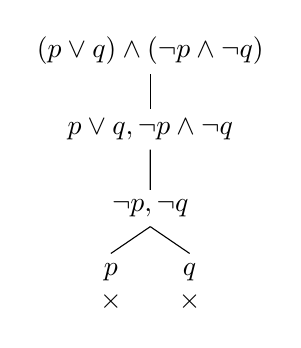
\begin{tikzpicture}[
        level distance=1cm,
        sibling distance=1.5cm,
        level 2/.style={sibling distance=1cm},
        edge from parent path={(\tikzparentnode.south) -- (\tikzchildnode.north)}
      ]
      \node {$(p \lor q) \land (\neg p \land \neg q)$}
        child { 
          node {$p \lor q, \neg p \land \neg q$}
          child { 
            node {$\neg p, \neg q$} 
            child { node[align=center] {$p$ \\ $\times$} }
            child { node[align=center] {$q$ \\ $\times$} }
          }
        };
      \end{tikzpicture}
      }  
    \end{latin}
    \end{center}
  با این حال، ما \emph{جدول معنایی کلاسیک} را ترجیح می‌دهیم زیرا در آن به‌وضوح دیده می‌شود که کدام فرمول‌ها نامزد تجزیه هستند و چگونه برگ‌ها علامت‌گذاری می‌گردند.
  
  \end{example}